\begin{secao}{Um Pouco Sobre a USP}

Vocês, que são novos na USP, devem saber desde cedo que aqui há muita
burocracia. É bom que se acostumem com ela, já que vocês terão que enfrentá-la.

O reitor é presidente do maior órgão da USP, o Conselho Universitário (abrevia-se
C.O. para evitar frases do tipo: ``Vou ter uma reunião no CU hoje'', ``O CU não
está funcionando muito bem esse semestre'', ``Os alunos não têm acesso ao CU''
etc.) que determina TODOS os rumos da universidade.

Abaixo dele vêm as coordenadorias e unidades. O SAS (Superintendência de Assistência Social),
por exemplo, é o departamento responsável pelos serviços
que a universidade oferece (não é a melhor coisa do mundo, mas oferece) para a
comunidade universitária: ônibus circulares, alimentação através dos restaurantes
universitários (famosos bandejões), moradia para estudantes (CRUSP) etc.

Alguns outros lugares que vocês devem saber que existem são o HU (Hospital
Universitário), o CEPE (Centro de Práticas Esportivas, leia ``cepê''), o banheiro
da FEA (Faculdade de Economia, Administração e Contabilidade), que fica na
frente do IME e é uma das faculdades mais bem abastecidas financeiramente
(apelidada ``carinhosamente'' de Shopping), a Física (certas aulas de laboratório são lá)
 e a querida Faculdade de Educação (para o pessoal da Licenciatura).

\begin{subsecao}{e-Disciplinas e E-mail USP}

Bixes, atenção e cuidado com o e-mail que vocês criaram (ou vão criar)! É um
email@usp.br, do sistema ``oficial'' de e-mails da USP, o que significa que é
através dele que a Universidade, o Jupiterweb, a diretoria do IME, o CAMat e
alguns desocupados lhes enviarão comunicados oficiais, o que pode envolver as
oportunidades diversas de intercâmbios, estágios, monitorias e tudo o mais que
vocês, simples bixes IMEanos, sejam capazes de se imaginar fazendo. Por este e-mail
vocês receberão informações antes mesmo que as principais sejam também colocadas
nos murais que ficam espalhados pelo IME (é, nem todas são colocadas em murais não).
Com as aulas on-line ou não, o e-mail sempre foi uma das principais formas de
comunicação (às vezes a única) entre nós alunos e todos os outros grupos, pessoas,
órgãos etc. que compõem as comunidades IMEana e da USP, então é sempre bom verificar
a caixa de entrada do seu e-mail com frequência! 

Além disso, peçam para os veteranes falarem mais um pouco de algumas 
(das \textbf{muitas}) vantagens de se ter um e-mail USP e aproveitem tudo aquilo que 
vocês agora têm direito!

A USP tem, há alguns anos, um ambiente virtual de aprendizagem para dar apoio
às disciplinas: o Moodle da nossa universidade, oficialmente conhecido como
e-Disciplinas (é comum chamarmos dos dois jeitos e há alguns professores que
se referem a ele como ``Stoa'', que é um nome bem antigo!). Você pode acessá-lo em
\url{https://edisciplinas.usp.br/}, fazendo login com o e-mail USP e a senha única.

Na página inicial, você provavelmente encontrará links para as páginas da maioria
das disciplinas que vai cursar (se não todas). Muitos professores não utilizam o 
e-Disciplinas como apoio aos seus cursos, às vezes fazem isso nos seus próprios 
sites institucionais ou simplesmente não usam a internet para nada. 

\end{subsecao}

\begin{subsecao}{Grupos no Whatsapp}

Com o intuito de organizar as atividades referentes a uma disciplina e ser uma
maneira prática e efetiva de passar recados, costumamos utilizar grupos do WhatsApp
para cada uma das matérias. Caso os links ainda não tenham sido criados,
vale a pena juntar seus amigos para criar os grupos no começo do semestre e espalhar
para os outros alunos.

Dentre as principais funções do grupo do WhatsApp estão:

\begin{enumerate}
%\item Colocar o link para acessar a plataforma on-line das aulas na descrição pra facilitar pra todo mundo;
\item Compartilhar os materiais e listas disponibilizados pelo docente da disciplina;
\item Passar recados importantes, sejam datas para entrega de trabalho, provas etc.;
\item Tirar dúvidas sobre a matéria com os coleguinhas.
\end{enumerate}

Pra ficar por dentro de tudo o que acontece na matéria, não se esqueça de procurar o
link e fazer parte dos grupos de whats das matérias que você está cursando!! :)

\end{subsecao}

\begin{subsecao}{Eduroam}

O Eduroam (EDUcation ROAMing, não tem nada a ver com alguém chamado Eduardo) é um
serviço de wi-fi que \sout{às vezes} provê acesso à Internet dentro de diversas
universidades (inclusive a USP). Mesmo que você seja aluno da USP, se viajar para
outra universidade, no Brasil ou no exterior, que possui o Eduroam, ainda poderá ter
acesso à Internet usando o mesmo login!

Para usar o Eduroam, basta se conectar à rede \texttt{eduroam}, colocando no campo
de login o seu número USP seguido por @usp.br. Por exemplo, se o seu número USP for
\texttt{123456789}, então deverá colocar no campo de login \texttt{123456789@usp.br}.
No campo da senha, deverá colocar a sua senha única (a mesma senha que vocês usam
para logar no Jupiterweb).

Tem várias outras informações sobre as configurações na hora de fazer login que
\sout{ninguém entende, mas se algum de vocês entender,} estão no site
\url{https://eduroam.usp.br/como-usar/}.

Para mais informações, acessem \url{https://eduroam.usp.br/}.

\end{subsecao}

\begin{subsecao}{O SAS}

A Superintendência de Assistência Social (SAS), que fica próxima à Praça do
Relógio, é o órgão da USP responsável pelo bem estar financeiro dos alunos — não
é lá a melhor coisa do mundo, mas ajuda... É onde vocês podem conseguir seus
milhares de benefícios, tais como auxílios financeiros, moradia gratuita (CRUSP)
ou auxílio alimentação (conhecido como vale-bandex) e dentistas gratuitos. Ou
seja, existem diversos tipos de auxílio e suporte. A SAS também é responsável
pelo Setor de Passes Escolares.

Se algum de vocês, bixes, estudou a vida inteira em escola pública, tem baixa renda,
sofreu agressões ou foi reprimido na infância, não pense que está sozinho nessa,
muitos também passaram por isso e vocês conseguem encontrar apoio aqui. Permanência
estudantil é um direito e não deve ser motivo de vergonha, portanto busquem
auxílio, pois podemos ajudar. Seguem as diversas alternativas para todos 
que precisarem:

\textbf{Moradia e auxílios financeiros}

Se vocês infelizmente não têm tanto acesso a meios de locomoção, ou dinheiro para
pagar transportes ou mesmo repúblicas, saibam que diversos auxílios podem ser
oferecidos para vocês para amenizar a sua situação:

% Com a carteirinha (e-card) que você recebeu na matrícula, você deverá entrar
% na página do SAS (\url{http://sites.usp.br/sas/}) e solicitar a inscrição
% para o processo de moradia e alojamento. Lá você terá um formulário, três
% trilhões de coisas para preencher e assim que te chamarem, deve apresentar os
% documentos (hum!) necessários para a assistente (você irá “ganhar” uma). Na
% improvável hipótese do site estar fora do ar, como todo ano acontece, você terá
% que ir ao SAS e pedir alojamento na USP, lá no Bloco G do CRUSP.

%REFTIME

As inscrições dos ingressantes para o Programa de Apoio à Permanência e Formação Estudantil (PAPFE)
deverão ser feitas dentro dos prazos estipulados no EDITAL PAPFE INGRESSANTES 2022, que pode 
ser encontrado na página do SAS (\url{https://sas.usp.br/wp-content/uploads/2022/02/editalIngressantes2022.pdf}).
No Portal de Serviços Computacionais da USP \url{https://portalservicos.usp.br/}, vocês entrarão 
com os dados da sua conta USP para se inscrever, responderão a questionários e anexarão (um bilhão de) 
documentos comprobatórios da situação socioeconômica declarada no ato de inscrição.

A prioridade é dada aos residentes de outros estados ou interior de São Paulo,
mas os moradores de São Paulo também podem solicitar, dadas as proporções da
cidade e o tempo de duas horas para que moradores da Zona Norte venham às aulas.

Vale ressaltar, bixes, que vocês tomem o cuidado de não fazer o mesmo que alguns
bixes de outros anos, que confundiram alojamento com o auxílio moradia (financeiro). São dois
requerimentos distintos e é bom que vocês fiquem atentos na hora de se inscrever, verificando
qual(is) tipo(s) de auxílio(s) vocês precisam.

Os requerimentos conterão perguntas sobre a situação socioeconômica, bem como os
documentos que deverão ser trazidos para comprová-la. Perguntas como renda
salarial, quantas pessoas contribuem com ela, números de bens móveis e imóveis,
situação habitacional, tipo de escola em que estudaram, se trabalham e há quanto
tempo, quanto gastam para vir à USP, o tempo de ida etc. Ainda há um espaço
para descreverem alguma particularidade não exposta nas perguntas que, obviamente,
receberá um parecer técnico.

Na classificação final da MORADIA, se vocês conseguiram uma pontuação grande, vocês
podem escolher entre a moradia no CRUSP ou um auxílio financeiro (bolsa moradia)
de R\$500,00 para vocês poderem alugar quartos, casas, hotéis, ou mesmo transporte
para ida e volta pra sua terra. Há casos em que a classificação final lhes permite
ter benefício apenas ao alojamento OU à bolsa, mas ao apartamento de três quartos
individuais (CRUSP) não.

Se vocês não conseguirem por nenhum desses meios, podem tentar a hospedagem, que é
simplesmente vocês ficarem no apartamento de alguém que more no CRUSP. Mas fiquem
atentos às datas de requerimento depois do resultado da seleção, pois vocês podem
ficar sem essa chance. Se mesmo assim vocês não conseguirem nada,
e acharem que os entenderam mal na entrevista ou coisa assim, vocês podem pedir para
entrar com recurso, e terem mais uma chance de esclarecer melhor a sua situação, ou também
procurar a AMORCRUSP (Associação dos Moradores do CRUSP, que fica no Bloco F, das 14h às 18h).

\textbf{Alimentação}

Vocês podem solicitar também o auxílio alimentação na página da SAS, que
consiste nos vale-bandex da USP e são válidos para almoço e jantar. Vocês deverão
passar por outra seleção que também inclui questionários socioeconômicos,
comprovantes, e mais papéis.

\textbf{Bolsa-trabalho}

Destina-se a alunos de graduação vinculados a projetos de extensão de serviços à
coletividade. Os projetos são selecionados anualmente, de acordo com sua relevância
para as finalidades da universidade pública e os estudantes vinculam-se por
afinidade acadêmica ou científica. Cada bolsa é de 1 (um) salário mínimo por
40 horas de trabalho mensais. Além da seleção socioeconômica feita pela
DPS (Divisão de Promoção Social), há uma seleção técnica feita pelos supervisores
dos projetos.

Mas fiquem espertos! Para tudo tem prazo e o SAS não é obrigado a ficar esperando a
boa vontade de aparecerem por lá de ninguém. Qualquer dúvida, liguem pro SAS.

\textbf{Atendimento odontológico gratuito}

Antigamente para vocês agendarem o atendimento odontológico gratuito era necessário fazer uma
carteirinha no HU (Hospital Universitário), em seguida comparecer ao Bloco G
do CRUSP com a carteirinha e agendar, porém hoje em dia, graças à tecnologia,
isso não é mais necessário: você só vai precisar mandar uns e-mails, preencher uns
formulários e esperar \sout{uma eternidade}.

Primeiro você precisa mandar um e-mail solicitando triagem para \url{triagemodonto.sas@usp.br},
vão te responder com um formulário que você vai preencher e enviar de volta, após isso eles
te colocarão na fila de espera pra triagem. No final, deve demorar muitos meses pra
eles te chamarem e quando fizerem isso você só vai ter que comparecer ao Bloco G do CRUSP
munido do seu cartão USP.

No final será demorado, porém o serviço é gratuito e realmente ajuda. Eles também atendem casos
de emergência como por exemplo dor de dente, algum dente quebrado ou qualquer outra situação
do gênero. No caso de dúvidas, são poucos os que podem te ajudar nesse assunto, então o melhor
a se fazer é ligar pra lá: (11) 3091-3393.

%FIXME
\textbf{Setor de passe escolar}

Será nesse lugar que você resolverá boa parte dos seus problemas com o SAS e com o
Bilhete Único. Você pode se dirigir ao Bloco “E” do CRUSP para receber orientação sobre
as mais diversas burocracias em que está se metendo.

Para as linhas da EMTU, SPTRANS, METRO, vocês devem entrar no site do SAS e fazer
o pré-cadastro para o respectivo cartão (\url {http://sites.usp.br/sas/}) para que a USP envie os 
seus dados para as empresas de transporte. Talvez demore um pouco, pois a USP tem que
avisar para a SPTrans que vocês passaram na Fuvest. Fiquem atentos! Qualquer dúvida,
liguem para a seção de passe escolar do SAS: (11) 3091-3581. Vocês também podem entrar nos sites 
das empresas de transporte e procurar por mais informações lá.

Há também um cartão especial para alunos de universidades públicas provenientes
de outras cidades do interior de São Paulo. Se algum de vocês vem de algum desses domos
ignotos (como Resende, Caçapava ou Guaíra), pode se dirigir ao guichê da sua empresa de
transporte intermunicipal (Cometa, Danúbio Azul etc.), apresentar seu Cartão USP,
preencher um formulário e eles aguardarão confirmação do seu instituto. Então
você pega seu cartão na Seção de Alunos e, na compra de passagens entre São Paulo
e sua cidade-natal, paga 50\% do valor normal. Só não deixe isto por último na
sua lista de necessidades porque existe um período do ano em que os guichês
liberam seus formulários; em resumo, espiche suas orelhas e corra para a rodoviária.

\end{subsecao}

\begin{subsecao}{Atendimento Psicológico}

Existem inúmeros serviços na USP que oferecem atendimento psicológico
aos alunos, cada um com um foco e um público-alvo. Dentre eles, existem 
aqueles oferecidos pelo Instituto de Psicologia (IPUSP) e pelo Escritório 
de Saúde Mental (ESM PRG).
Os principais serviços do IP são o LEFE, o Atendimento Presencial e o PAPO:

O LEFE se trata de um plantão psicológico oferecido à comunidade, em que
você pode conversar com um profissional num momento de crise. O plantão 
funciona na terça-feira às 17 h, no IP, e para ser atendido basta chegar 
entre as 16 e 17 h.

Mais informações sobre o LEFE: 
\url{https://www.ip.usp.br/site/plantao-psicologico-lefe/}

O Atendiento Presencial no IP é o serviço em que você pode ter acesso a
atendimento individual de forma contínua por um período mais longo. Essa
modalidade também exige inscrição, e os inscritos ficam em uma lista para
passar por triagem. O período com maior chance de ser selecionado é no inicio
do semestre, mas também é possível conseguir vagas em outros momentos em 
situações excepcionais. 

Mais informações sobre o Atendimento:
\url{https://www.ip.usp.br/site/atendimento-4/}

O PAPO é o Projeto de Apoio Psicológico Online, que foi criado durante a 
pandemia para oferecer de forma segura uma via de atendimento psicológico
para a comunidade. Para essa modalidade de atendimento é preciso se inscrever
previamente, no período indicado no site.
\url{https://www.ip.usp.br/site/covid-19-apoio-psicologico-online/}

O IP também oferece outros serviços, como o Ateliê Aberto e o Serviço
de Orientação Profissional. Você pode conhecer eles aqui:
\url{https://www.ip.usp.br/site/centro-escola-do-instituto-de-psicologia-da-usp-ceip/}

Além daquilo que foi listado acima, você também pode procurar o Escritório de Saúde
Mental, que oferece um serviço de acolhimento em três sessões, e pode encaminhar
os casos em que houver necessidade para outros serviços. O contato é feito pelo
formulário que se encontra no link:
\url{https://prg.usp.br/escritorios-prg/esm-escritorio-de-saude-mental/}


Bixes, sempre que precisarem, não tenham receio de procurar apoio
psicológico, por mais banal que vocês possam achar o motivo. Vocês
podem frequentar os serviços oferecidos pela USP para conversar sobre
qualquer coisa que esteja lhes incomodando, sejam professores,
matérias, EPs ou algo do tipo sem criar qualquer
problema para vocês no IME.

\end{subsecao}
\pagebreak
% Utilize para começar uma nova página do lado esquerdo do Guia!

\begin{subsecao}{Bandejão}
%TODO Fazer as duas páginas ficarem na mesma "visualização" no guia impresso
%Ou seja, usar esquema Odd/Even do LaTeX.
% Isso foi deixado de lado nessa versão de 2016 para que o mapa dos circulares
% ficasse no lugar certo e não tivesse nenhuma página em branco
% (como o cleardoublepage ali em cima)
% 2017: não sei se entendi o que era para ser feito, mas usei o
%       \cleardoublepage para a imagem do calvin não ficar zuada.


Os bandejões, vulgarmente conhecidos como Restaurantes do SAS, são os lugares
em que vocês podem se alimentar razoavelmente a um preço analogamente razoável.
Os tickets custam R\$ 2,00, sendo estes carregados na carteirinha USP. O
lugar para carregar o ``bandejão único'' é no CARE (Centro USP de Acolhimento e 
Referência para Estudantes), perto do SAS e do bandejão Central. Além disso, é 
possível verificar o saldo atual e comprar mais créditos via boleto ou Pix no site
{\tt https://uspdigital.usp.br/rucard/} ou pelo aplicativo ``Cardápio+ USP'',
disponível para Android e iOS (não se esqueça de olhar também os outros
aplicativos da USP disponíveis, pois podem ser muito úteis).
É uma ótima alternativa para evitar as infinitas filas dos guichês de venda. Os
créditos demoram até 03 (três) dias úteis para estarem disponíveis, caso vocês
paguem via boleto. Se realizarem o pagamento pelo Pix, os créditos podem ser usados
dentro de alguns minutos.
Dica: Confira o saldo da carteirinha no site ou no aplicativo antes de tentar usar!

Existe uma lenda que sobremesas especiais aparecem em certos bandejões perto de
datas comemorativas. Mas não se engane - normalmente, elas não aparecem no
cardápio (talvez para não ficar muito cheio de gente).

\figuragrande{bandex_calvin}

O cardápio semanal do bandejão pode ser visto no site {\tt
http://sites.usp.br/sas/} ou pelo aplicativo ``Cardápio+ USP'', mas se vocês
estiverem com preguiça de ver em um desses lugares, é bem provável que um veterane 
já saiba e resolva informar, se questionado com muita educação.

O cardápio é geralmente composto de arroz (com opção normal e integral), feijão,
prato principal (carne/ovos), acompanhamento (legumes ou verduras refogadas,
cremes, molhos), salada (algumas folhas), sobremesa (frutas e/ou, às vezes, algo mais
requintado), pãozinho (normal e integral) e suco (de diversos sabores: azul, vermelho,
amarelo, etc.), além de temperos genéricos (jamais perguntem do que eles são feitos). 
Se vocês são vegetarianos, o acompanhamento nunca contém carne (e estão tentando 
fazer com que sejam veganos também), e todos os bandejões têm uma alternativa 
vegetariana de PVT para o prato principal, normalmente vindo na forma de ração,
mas existindo as formas de lasanha, kibe, e outros.


Não se esqueçam de levar as suas canecas do Kit-bixe se forem comer nos
bandejões, tanto para ostentar a posição de bixes do IME, quanto para salvar o
meio ambiente, evitando assim o uso de copos descartáveis. Os badenjões não 
disponibilizam copos e não aceitam o uso de garrafas nas máquinas de suco, por 
isso, é muito importante que vocês sempre tenham um copo ou caneca para conseguir 
tomar o líquido colorido saborizado do bandeco.


PS: O Efeito Bandex é proporcional à quantidade de salitre utilizado em cada
bandejão.\\
PS 2: Nunca, em hipótese alguma, jamais, visite a cozinha do seu bandejão de
preferência, pois você corre o risco de nunca mais almoçar na vida. Como já
dizia o velho sábio ``A ignorância é uma virtude''.\\
PS 3: Playstation 3.

Consultem a tabela abaixo para decidir em qual dos bandejões vocês vão comer.

\begin{figure}[!htbp]
\begin{center}
 	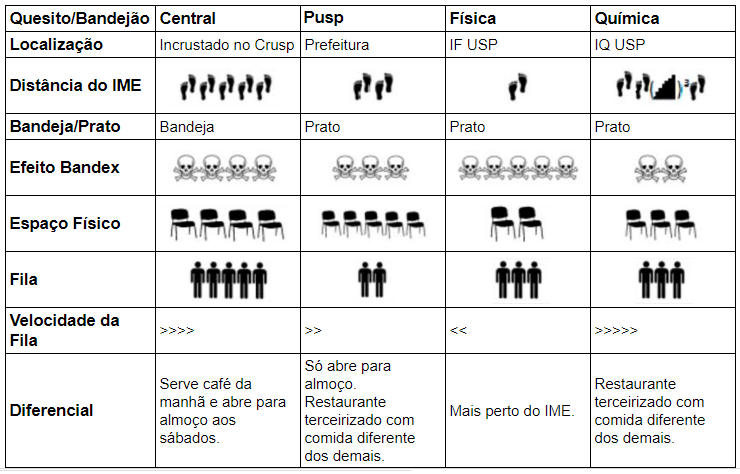
\includegraphics{img/src/tabela_bandeco.png}
\end{center}
\end{figure}


O horário de funcionamento dos bandejões é o seguinte:
\textbf{Café da manhã:} 7h às 8h30min (somente no Central, de segunda à sábado)\\
\textbf{Almoço:} 11h15min às 14h15min (em todos os bandejões de segunda à sexta, de sábado 
somente do Central e de domingo somente na Química)\\
\textbf{Jantar:} 17h30 às 19h45 (somente na Química, na Física e no Central de segunda à sexta)\\

IMPORTANTE: o funcionamento dos bandejões pode ser alterado ao decorrer do ano,
principalmente nos feriados, por isso recomendamos que vocês fiquem atentos ao 
aplicativo e às placas informativas presentes nos bandejões.

Para mais informações, visitem o site do SAS: \url{http://sites.usp.br/sas/} ou
utilizem o aplicativo ``Cardápio+ USP''.

\end{subsecao}

\begin{subsecao}{Outros lugares para comer na USP}

Caso vocês, bixes, não queiram comer no bandejão, seja porque estão com medo do
prato do dia ou simplesmente porque querem comer algo diferente (e
possivelmente de sabor melhor), saibam que há alguns outros lugares na USP onde
vocês podem comer; por exemplo, os que estão nesta lista.

%REFTIME
Importante: grande parte das informações a seguir não está tão certa porque já
fazem (pelo menos) três anos que verificamos pela última vez, então sempre que estiver
escrito ``custa R\$ $x$'' interpretem como ``vai custar um tanto a mais que R\$ $x$''.

\textbf{Lanchonete da Física}

Fica um pouco antes do bandejão da Física, nela vocês podem almoçar pagando R\$
40,90 o quilo, sempre tem uma razoável quantidade de saladas e pratos
quentes, além disso, tem churrasco com uma boa variedade de opções.
Além do almoço por quilo, lá vende alguns salgados e lanches como sanduíches e
beirutes. E um pouco antes da lanchonete, há um lugar que vende cookies por R\$
3,50 (3 unidades). Vocês vão sentir o cheiro dos cookies quando forem bandejar.

\textbf{Restaurante do IPEN}

Fica na parte de cima da rua entre o IF e o Parque Esporte Para Todos, para
entrar lá vocês precisam da carteirinha USP. Lá o quilo é R\$ 24,50, porém não
tem uma variedade muito grande de comida, tem marmitex também que é R\$ 11,70.
Ele só abre para pessoas de fora às 13h e antes de ir para o restaurante vocês
devem se identificar.

\textbf{Lanchonete da FAU}

Localizada dentro da FAU assim que você sobe a rampa. Lá além de lanches é
servido almoço tanto por quilo (custa R\$ 43,90) como prato feito. Tirando o por
quilo, qualquer outra coisa deve ser paga no caixa antes de retirar. Além
disso, no terceiro andar da FAU tem a mesinha de doces que os alunos deixam lá
para vender, a variedade e quantidade de doces varia bastante com o dia e o
preço deles costuma ser no máximo R\$2,50.

\textbf{Restaurante da FEA}

Fica atrás da FEA, lá o quilo tem bastante coisa diferente e algumas até que
sofisticadas, porém o preço do quilo lá é R\$61,90, provavelmente é o mais caro
da USP. Geralmente é frequentado por professores e funcionários da USP. Além do
self-service, há algumas opções de prato feito que custam R\$22,00.

\textbf{Trailers de lanche da \sout{ECA} Química}

Ficam na calçada com a Avenida Lineu Prestes, em frente ao Instituto de
Química. Nesses carrinhos vende pastel, sanduíches, churros, tapioca e salgados
em geral. Os preços dos lanches variam entre R\$3,00 e R\$10,00. As opções de
sanduíches e a quantidade de sabores de tapioca é bem grande e todos em geral
são muito bons. Já o pastel você pode escolher de 1 a 5 ingredientes para pôr
no pastel, portanto o preço varia de acordo com a quantidade de ingredientes que
vocês vão querer.

\textbf{Cachorro-quente da Reitoria}

Fica na rotatória da biblioteca Brasiliana (ou a rotatória depois do CEPE, se assim preferir),
lá o cachorro-quente pode ser feito tanto no pão de cachorro-quente como na baguete. Além disso,
há a opção de pôr catupiry e de pôr uma salsicha adicional. O preço do cachorro-quente varia
entre R\$9,00 e R\$12,00.

\textbf{Poke da Reitoria}

Tem um lugar que vende Poke (um prato havaiano que mistura peixe cru em cubos,
arroz, shoyu e frutas) ao lado do cachorro-quente. Esta iguaria custa
aproximadamente R\$23, e você pode escolher os ingredientes que vão no seu prato,
tipo Spoleto. Dá pra fazer um Poke vegano, com cogumelos em vez de peixe. Além de
Poke, também vende Temakis, Hot Rolls, e até Açaí. A qualidade é boa, mas as filas
podem ser demoradas.

\textbf{Pastel do IEE}

Esse lugar maravilhoso fica a apenas alguns passos do IME. Apenas às terças-feiras,
em um canto escondido do IEE (pergunte a um veterane como chegar!) fica o famoso pastel do IEE.
Há muitas opções de sabores, além de poder comprar um caldo de cana para acompanhar (também tem várias opções de sabores!).

\end{subsecao}

\end{secao}
